\documentclass{article}
\usepackage{spconf,amsmath,graphicx, bbm}
\usepackage{tabularx}
\usepackage{multicol} 
\usepackage{multirow}
\usepackage{booktabs}
\usepackage{hyperref}
\usepackage{url}
\usepackage[toc,page]{appendix}
\usepackage{subfig}
\usepackage{subcaption}
\usepackage{ragged2e}
\captionsetup{compatibility=false}
\title{the methodology for stereo image learning representation}

\name{Seongrae Kim$^{\star}$ \qquad Changwoon Choi$^{\dagger}$ \qquad Sangwoo Han$^{\ddagger}$}
\address{$^{\star}$ Mechanical Engineering, Seoul National University \\ $^{\dagger}$ Electrical \& Computer Engineering, Seoul National University \\$^{\ddagger}$ Earth \& Environmental Sciences, Seoul National University}

\begin{document}
\maketitle

\begin{abstract}
In this work, we present an audio generative model which is able to produce ... 
\footnote{Dataset and code are available on \url{https://github.com/changwoonchoi/ml2020}}
\end{abstract}

\begin{keywords}
Generative model, Multi-channel audio, Learning representation
\end{keywords}

\section{Introduction}
\label{sec:intro}

\if 0
Blahblah

Overall, we propose an $\cdot$. We show promising results on stereo audio generation problem with our new dataset. In summary, the main contributions of this work are:
\begin{itemize}
    \item 
    \item 
    \item 
\end{itemize}
\fi
\section{Related Work}
\label{sec:related_work}
\subsection{Audio generative model}
The earliest generated models for audio tend to focus on speech synthesis. In this case, models require handling variable length, and WaveNet~\cite{wavenet} used the autoregressive method for variable-length inputs and outputs. A flow-based WaveGlow~\cite{waveglow} has emerged that compensates for slow speed of autoregressive models. In comparison to speech, audio generation for music is relatively in the development stage. ~\cite{nsynth} proposed generation of a single musical note to use WaveNet, but it is still slow, and global latent conditioning was impossible. GANSynth~\cite{gansynth} with Generative Adversarial Network solves these shortcomings and provides high-fidelity and locally-coherent audio represented with log magnitudes and instantaneous frequencies with sufficient frequency resolution in the spectral domain. As a result of the research to date, it is possible to learn a single note of a variety of instruments to convincingly describe the sound of real instruments and to create a variety of synthesizers by interpolation between two instruments. Despite such breakthrough development, the reason that the generated musical notes cannot be used for commercial music is that the generated result is a single channel. Despite this breakthrough, the generated musical notes cannot replace commonly used virtual instruments due to the limitation of a single channel.

\subsection{Multi-channel audio}

In the machine listening community, multi-channel audios are mainly used for speech separation~\cite{multi_ch_sourcesep}, speech enhancement~\cite{speech_enh}, and speech recognition~\cite{speech_recog} in the light of their ability to utilize information about speech source location. On the other hand,~\cite{upmix} proposed an upmixing conversion of the mono signal to pseudo-stereo in order to enhance the audio effect. However, to the best of our knowledge, there are still no attempts to generate high-fidelity multi-channel audio with a neural network. It is necessary to learn the difference while maintaining the coherency of both channels to form a spatiality of sound. A technique referred to as “mid-side coding” exploits the common part of a stereophonic input signal by encoding the sum and difference signals of the two input signals rather than the input signals themselves. (~\cite{mscoding} described the concept of mid-side coding of using the interchannel redundancies.) Therefore, for a high-performance multi-channel audio generative model, we would like to train the state-of-the-art audio generative model(~\cite{gansynth}, so-called GANSynth) through the mid-side coding to verify whether this attempt can effectively learn stereo image.
\section{Proposed Method}
\label{sec:method}

\section{Experiments}
\label{sec:experiment}

In this section, we first propose our novel representation of stereo audio, \textit{`Side distance' ($D_{side}$) and `Short-time Side Distance (STSD)'}. Next, we introduce existing metrics for evaluating sample generation, then propose our new metrics for evaluating stereo image generation by combining existing metrics with side distance and STSD. We then compare the proposed method using M-S channels with the previous method(GANSynth~\cite{gansynth}) which consumes L-R channels by both quantitative and qualitative methods.

\subsection{Representation for stereo audio}
\label{subsec:representation}
The goal of the generative model is to learn to produce samples that look similar to the ones on which it has been trained. Therefore, in order to evaluate the generative model, a proper distance metric between the generated samples and the samples from the dataset is essential. Until now, however, a metric for measuring the similarity between stereo images has never been suggested. In this section, we propose a novel representation of stereo audio that allows us to define the distance metric between them.

\subsubsection{Side distance}
\label{subsubsec:side_distance}
\begin{figure}[t]
    \centering
    \subfloat[SD]{
    \label{subfig:SD}
    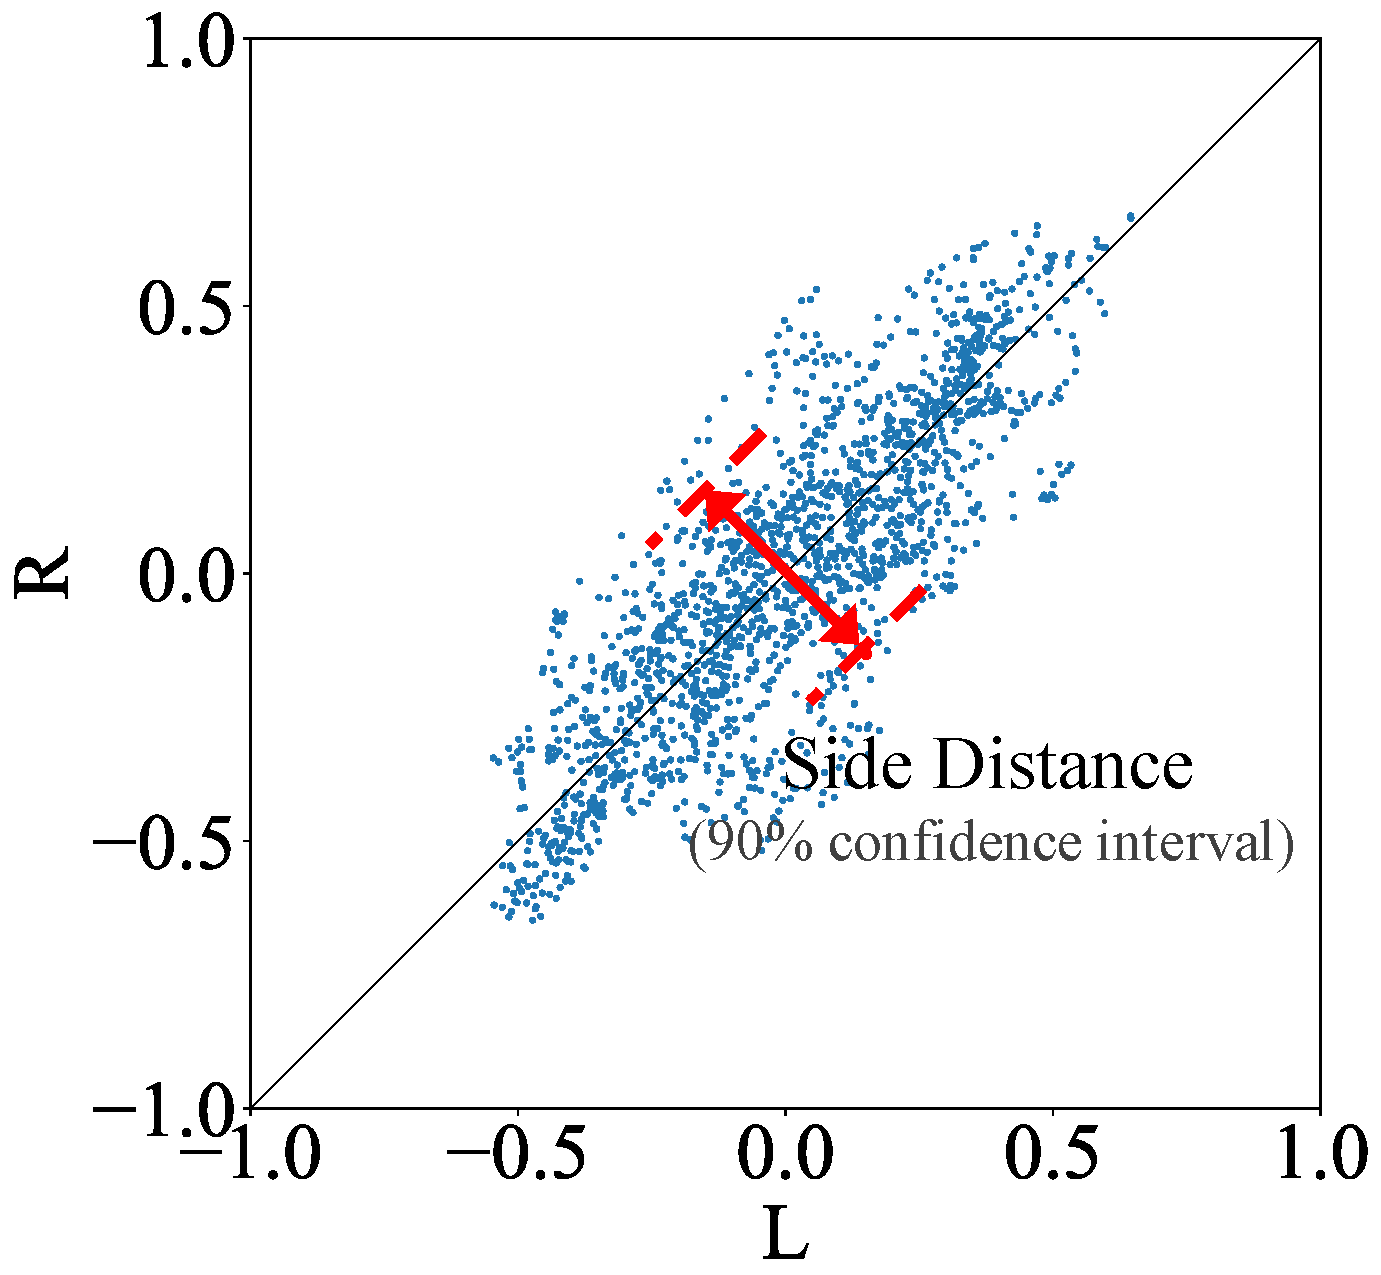
\includegraphics[width=0.69\linewidth]{assets/figures/scatter_38.pdf}
    }
    \subfloat[STSD]{
    \label{subfig:STSD}
    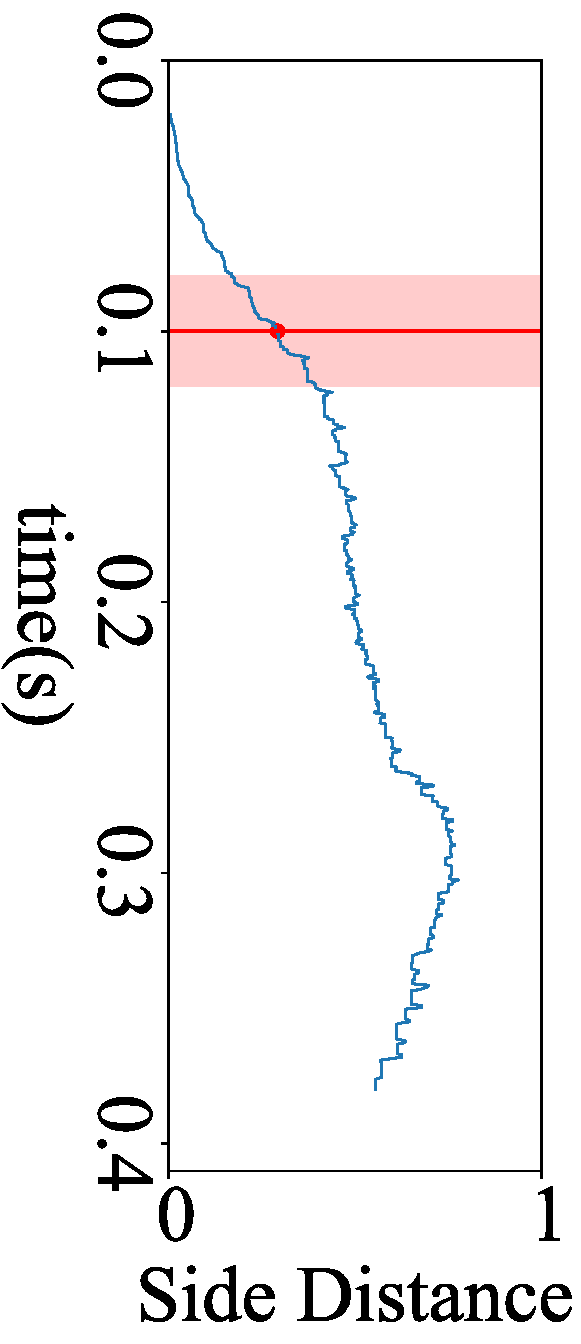
\includegraphics[width=0.28\linewidth]{assets/figures/stsd_38.pdf}
    }
    \caption{caption}
    \label{fig:stsd}
\end{figure}
When $y$ is a stereo audio of length $T$, we define \textit{`side distance'} $D_{side}$ as following:
\begin{equation}
    D_{side}(y) = {\frac{\sqrt{2}}{2}}(\max_{t \in [0, T)} [y_L(t) - y_R(t)] - \min_{t \in [0, T)} [y_L(t) - y_R(t)])
\end{equation}
where $y_L$ and $y_R$ are left and right channel of stereo audio $y$. For robustness, we use the 0.95, 0.05 quantiles of $y_L(t) - y_R(t)$ instead of maximum and minimum. The side distance can be viewed as an index indicating how far the given stereo audio is spread as visualized in Fig.~\ref{subfig:SD}

\subsubsection{Short-time Side Distance (STSD)}
\label{subsubsec:stsd}
Although side distance is an indicator of how wide the given stereo audio is spread in the auditory space, it cannot express the change of the stereo image over time. Therefore, we introduce the concept of \textit{`Short-time Side Distance (STSD)'} to capture the characteristics of the stereo image over time. The STSD is a sequence of side distance of a windowed signal. The procedure to obtain STSD is to divide a longer time signal into shorter segments of equal length and then compute side distance on each shorter segment. Formally,
\begin{equation}
    STFT(y(t)) = D_{side}(y(\tau)w(t))
\end{equation}
where $w(t)$ is a window function which is nonzero for short period of time. As depicted in Fig.\ref{subfig:STSD}, STSD contains the change in the side distance of the windowed short fragment of signal over time.
\subsection{Evaluation metrics}
\label{subsec:metric}
Following prior work, we use earth mover's distance (EMD), proposed by~\cite{emd} to measure the similarity between two stereo audios' STSDs. Formally, EMD is defined as follows:
\begin{equation}
    \text{EMD}(s_1, s_2) = \min_{\phi: s_1\to s_2} \sum_{x\in s_1} \|x-\phi(x)\|_2 \nonumber
\end{equation}
where $s_1$ and $s_2$ are two distributions and $\phi$ is a bijection between them. Note that $s_1$ and $s_2$ can be any distribution. One can use STSD of stereo audio as $s_1$ and $s_2$.

Let $S_g$ be the set of generated stereo audios and $S_r$ be the set of reference audios with $|S_g| = |S_r|$. To evaluate generative models, we consider the three metrics, MMD, COV which are introduced by~\cite{achlioptas} and 1-NNA proposed by~\cite{1-nna}.

\begin{itemize}
	\item\textbf{Coverage (COV)} measures the fraction of stereo audios in the reference set that are matched to at least one stereo audio in the generated set. For each stereo audio in the generated set, its nearest neighbor in the reference set is marked as a match:
	\begin{align*}
	\text{COV}(S_g, S_r) = \frac{|\{\arg\min_{Y \in S_r} D(X,Y) | X \in S_g \}|}{|S_r|},
	\end{align*}
	where $D(X,Y)$ is a distance metric between two stereo audios.
	While coverage can detect mode collapse, it does not evaluate the quality of generated stereo audios. 
	\item\textbf{Minimum matching distance (MMD)} is proposed to complement coverage as a metric that measures quality. For each stereo audio in the reference set, the distance to its nearest neighbor in the generated set is computed and averaged:
	\begin{equation}
	\text{MMD}(S_g, S_r) = \frac{1}{|S_r|}\sum_{Y\in S_r} \min_{X\in S_g} D(X,Y),\nonumber
	\end{equation}
	where $D(X,Y)$ is a distance metric between two stereo audios.
	\item \textbf{1-nearest neighbor accuracy (1-NNA)} is proposed by Lopez-Paz and Oquab~\cite{1-nna} for two-sample tests, assessing whether two distributions are identical.
	Let $S_{-X} = S_r \cup S_g - \{X\}$ and $N_X$ be the nearest neighbor of $X$ in $S_{-X}$. $1$-NNA is the leave-one-out accuracy of the 1-NN classifier with given distance metric:
	\begin{align*}
	\text{1-NNA}(&S_g, S_r) \\
	=&\frac{\sum_{X\in S_g} \mathbbm{1}[N_X \in S_g] +  \sum_{Y\in S_r} \mathbbm{1}[N_Y \in S_r]}{|S_g|+|S_r|} ,
	\end{align*}
	where $\mathbbm{1}[\cdot]$ is the indicator function.
	For each sample, the 1-NN classifier classifies it as coming from $S_r$ or $S_g$ according to the label of its nearest sample.
	If $S_g$ and $S_r$ are sampled from the same distribution, the accuracy of such a classifier should converge to $50\%$ given a sufficient number of samples. The closer the accuracy is to $50\%$, the more similar $S_g$ and $S_r$ are, and therefore the better the model is at learning the target distribution.
\end{itemize}
As a definition of COV, MMD, 1-NNA, and $D(X,Y)$ can be any distance metric between two audio samples. We use EMD(STSD($X$), STSD($Y$)) as a distance metric $D(X,Y)$.

\subsection{Experimental results}
\label{subsec:result}
\if 0
\subsubsection{Dataset}
\label{subsubsec:dataset}
In this work, we propose a new dataset contains stereo audios with rich stereo images. The dataset consists of EDM stabs with 400ms time duration. Further details can be found in Appendix~\ref{sec:dataset_detail}. 
\fi

\subsubsection{Quantitative results}
\label{subsubsec:result}
\begin{table}[t]
    \centering
    \begin{tabular}{l|c|c|c}
        \toprule
         & COV ($\uparrow$) & MMD ($\downarrow$) & 1-NNA ($\downarrow$)\\
         \midrule
         LR & 34.55 & 1.42 & 76.22 \\
         MS & 45.31 & 1.05 & 68.66 \\
         \bottomrule
         
    \end{tabular}
    \caption{Quantitative comparison results of stereo generation on \textit{datasetname}.
    	The best results are in bold.
    	Note that MMD is multiplied by $10^3$. }
    \label{table:result}
\end{table}

\if 0
\begin{table}[t]
\centering
    \begin{tabular}{c|cc|cc|cc}
		\toprule
		 & \multicolumn{2}{c|}{COV ($\uparrow$)} & \multicolumn{2}{c|}{MMD ($\downarrow$)} &  \multicolumn{2}{c}{1-NNA ($\downarrow$)}\\
		\midrule
		Epoch & \multicolumn{1}{c|}{LR} & \multicolumn{1}{c|}{MS} & \multicolumn{1}{c|}{LR} & \multicolumn{1}{c|}{MS} & \multicolumn{1}{c|}{LR} & \multicolumn{1}{c}{MS} \\
		\midrule
		50&  1.04 & 1.27 & - & - & - & - \\
		100&  - & - & - & - & - & - \\
		150&  - & - & - & - & - & - \\
		200&  - & - & - & - & - & - \\
		\bottomrule
	\end{tabular}
    \caption{
    	Quantitative comparison results of stereo generation on \textit{datasetname}.
    	The best results are in bold.
    	Note that MMD is multiplied by $10^3$. 
    }
    \label{table:result}
    
    % \vspace{-1em}
\end{table}
\fi
For a fair comparison, we trained both our model and GANSynth~\cite{gansynth} with exactly same the hyperparameters (including network architectures, learning rate, epochs) in our training set. The only difference during the training scheme between GANSynth~\cite{gansynth} and the proposed method is the channel encoding. Our proposed method consumes two-channel audio that is reparameterized from L-R representation to M-S representation while GANSynth~\cite{gansynth} takes input as raw L-R represented stereo audios. The quantitative results are reported in Table~\ref{table:result}. We observe that it is improved significantly by simply reparameterize the stereo audio in terms of every evaluation metrics (COV, MMD, 1-NNA).
\vspace{-0.5em}

\subsubsection{Comparing audio quality to concurrent work}
\label{subsubsec:audio_quality}
\begin{figure}[t]
    \centering
    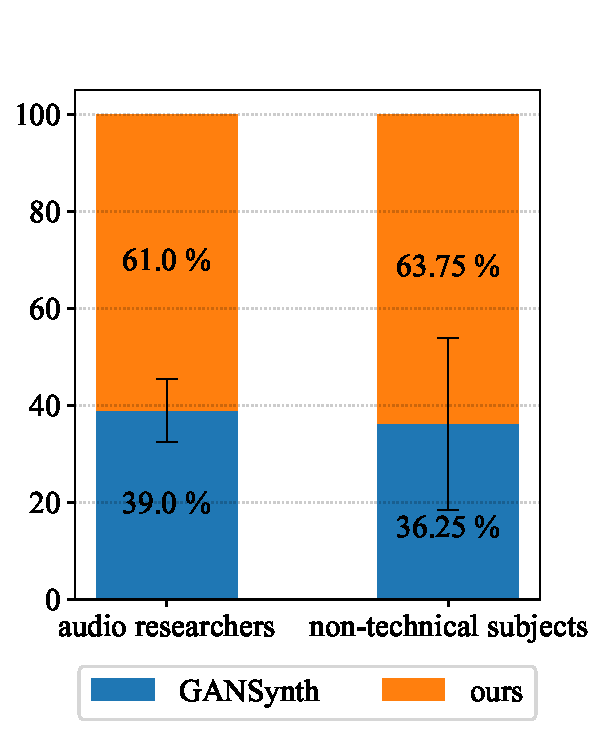
\includegraphics[width=0.8\linewidth]{assets/figures/quality_result.pdf}
    \caption{Listening evaluation for audio quality to concurrent work. Our method received better results on both subject group, especially it is quite significant for audio researchers group ($p < 0.01$).}
    \label{fig:quality_result}
\end{figure}
To better compare our method with concurrent work, we perform a subjective analysis over the stereo audios generated by both methods. In Fig.~\ref{fig:quality_result}, we show the percentages of participants based on how they voted for the plausibility comparisons between ours and GANSynth~\cite{gansynth}. The study employed 15 participants with different backgrounds - 5 audio researchers, 10 non-technical subjects. The participants are asked to choose the better audio between ours and other work. We can observe that our method received better results on both the audio researcher group and the non-technical subject group.
\vspace{-0.5em}
\section{Conclusion}
\label{sec:conclusion}

\bibliographystyle{IEEEbib}
\bibliography{our_bib}
\appendix
\section*{Appendix}
\section{Additional Implementation Details}
\subsection{Neural Network Architecture}
\subsection{}
\section{Dataset Details}
\section{Evaluatin Metrics}
\end{document}
